\chapter{提案手法} \label{chap:method}
%%%%%%%%%%%%%%%%%%%%%%%%%%%%%%%%%%
%    3Dモデリングにおけるエンティティ
%%%%%%%%%%%%%%%%%%%%%%%%%%%%%%%%%%
\section{データ構造}
サーバのデータを従来のテキストと同様に一次元に管理すると, 依存関係があった場合にデータの管理が困難となる.
3Dモデリングで用いるエンティティごとにデータを作成し, そのデータモデル間で依存関係を持つことによって解決する.
本システムでは3Dモデリングで用いるオブジェクト, 面, 頂点の3つのデータを定義し, 新しくデータを作成する場合, データベースにデータを登録していく仕様にした.
また, サーバデータとそのデータを各クライアントにコピーしたシャドウコピーを区別するために, シーンというデータを定義する.
図\ref{データ構造}にデータモデル間の依存関係を表した図を示す.
\begin{figure}[htbp]
  \begin{center}
    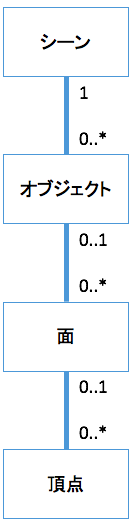
\includegraphics[scale=0.5]{images/er}
    \caption{データモデル間の依存関係}
    \label{データ構造}
  \end{center}
\end{figure}
図\ref{データ構造}のようにシーンのデータはオブジェクトを, オブジェクトは面を, 面は頂点をそれぞれ子にもつ. また, 子のみが親の参照先をもつ.

このデータ構造によって, 子を削除した場合に親との依存関係も削除できる.親を新しく設定する場合, 子のデータを複製しながらそれぞれに新しく設定する親を参照先に設定する.
子のデータを複製していくことによって, 関係を削除した際も複製元のデータは残る.
%%%%%%%%%%%%%%%%%%%%%%%%%%%%%%%%%%
%    固有IDの付与
%%%%%%%%%%%%%%%%%%%%%%%%%%%%%%%%%%
\section{固有IDの付与} \label{固有id}
各データには, 複数クライアント間でIDの衝突が起こるのを防ぐため, そのデータを作成したクライアント識別子を組み込んだ固有IDを与える.
本システムでは図\ref{uuid}のように, クライアント識別子--データモデル識別子--インクリメント番号--ランダム文字列の順につなげた固有IDを与えた.クライアント識別子は1から順に振られたユーザIDを用いてクライアントが付与するように決め, 初期データはシステムが作ったということで0を与えた. また, オブジェクトは0, 面は1, 頂点は2ということでデータモデル識別子を与えた. サーバでもクライアントでも作ったデータの数を記憶しておき, 作るごとにインクリメントするインクリメント番号を固有IDに組み込んだ.
\begin{figure}[htbp]
  \begin{center}
    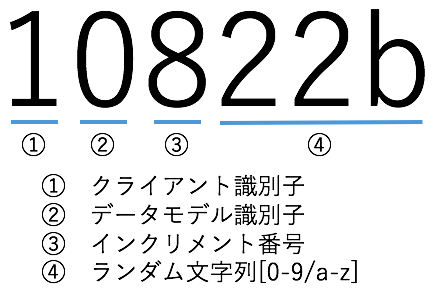
\includegraphics[scale=0.5]{images/uuid}
    \caption{本システムの固有ID}
    \label{uuid}
  \end{center}
\end{figure}
%%%%%%%%%%%%%%%%%%%%%%%%%%%%%%%%%%
%    基本命令
%%%%%%%%%%%%%%%%%%%%%%%%%%%%%%%%%%
\section{基本命令} \label{ope}
オブジェクト, 面, 頂点の各データモデルに対して, 作成, 親への参照の追加, 削除の3つの基本命令を実装した.
これらの命令はシステムに対する最低限の基本命令であり, これらの命令を組み合わせることで, 3Dモデリングで使われる面の分割や押し出しなど, より高度な命令を実現できる.
削除命令や親への参照の追加をする命令を適用する際, 操作対象が他の命令で削除されていた場合は命令を無効とする.
%%%%%%%%%%%%%%%%%%%%%%%%%%%%%%%%%%
%    クライアント接続時
%%%%%%%%%%%%%%%%%%%%%%%%%%%%%%%%%%
\section{クライアント接続時の処理}
あるクライアントが初めて接続した場合, そのクライアントの識別子を持ったシーンのデータを作成する. このシーンのデータが, Differential Synchronizationにおいてそのクライアントのサーバシャドウになる. このあるクライアントが初めて接続した際, サーバデータとの差分を出すために, サーバシャドウはオブジェクトの情報を持たない. サーバデータとの差分を計算した後, シャドウコピーを行う.
%%%%%%%%%%%%%%%%%%%%%%%%%%%%%%%%%%
%    シャドウコピー
%%%%%%%%%%%%%%%%%%%%%%%%%%%%%%%%%%
\section{シャドウコピー}
本来, 変数v1を変数v2にシャドウコピーするならばv2 = v1のように代入することで実装する. しかし, 本システムではデータをデータベースに登録して管理しており, 単純な代入で処理できない.
また, 元のデータを削除し新しくシャドウコピーを作成する方法は, 頻繁にシャドウコピーを行うDSでは,
データベースのDELETE命令とCREATE命令を頻発させることになり, 処理においてボトルネックとなってしまう. サーバデータとサーバシャドウの差分を取り, サーバシャドウに適用することによってシャドウコピーを作り解決する.
